\section*{4 Experiments}
We evolve harnesses for a frozen Qwen3-4B executor~\citep{qwen3} on ALFWorld~\citep{alfworld}, WebShop~\citep{webshop}, and DBBench and OSBench from AgentBench~\citep{agentbench}. We report best measured checkpoint test success, with sample standard deviations over repeated executions. Appendix~B describes the A/B/C experimental setup. Appendix~D defines the metrics.

\paragraph{Edit scope.}
A, B, and C progressively expand what the improver can change in a harness. A revises skill text. B also exposes memory, action checks, and tool feedback, with one independent component edited per candidate. C allows coordinated changes to executable plugins and shared episode state. A single C candidate can connect a tool receipt to later context and action checks.

\FloatBarrier
\subsection*{4.1 Benchmark Results}
\suppressfloats[t]
\begin{table*}[!htbp]
\centering
\caption{Test success with a Qwen3-4B executor across four benchmarks}
\label{tab:main-results}
\begingroup
\setlength{\tabcolsep}{1.4pt}
\renewcommand{\arraystretch}{1.08}
\fontsize{8.5}{10}\selectfont
\begin{tabularx}{\textwidth}{@{}p{0.32\textwidth}*{4}{>{\centering\arraybackslash}X}@{}}
\toprule
Method & ALFWorld & DBBench & WebShop & OSBench \\
\midrule
\rowcolor{grouphead}\multicolumn{5}{l}{\textbf{Local evaluations}} \\
\rowcolor{ourrow}\textbf{Ours: Sol high (measured peak)} & \textbf{95.41$\pm$0.00} & \textbf{70.56$\pm$0.38} & \textbf{48.17$\pm$0.29} & \textbf{41.67$\pm$1.84} \\
Life-Harness (local)\citep{life} & 87.77$\pm$1.91 & 64.11$\pm$0.38 & 41.33$\pm$0.29 & 36.81$\pm$0.00 \\
\addlinespace[3pt]
\rowcolor{grouphead}\multicolumn{5}{l}{\textbf{Published comparisons with Qwen3-4B}} \\
Life-Harness (v3)\citep{life} & 88.07 & \underline{65.00} & \underline{45.50} & \underline{39.60} \\
Bare\citep{life} & 16.51 & 44.00 & 29.50 & 21.50 \\
ALIGN\citep{align}\citep{life} & 28.36 & — & 18.00 & — \\
AgentSquare\citep{agentsquare}\citep{life} & 29.36 & — & 18.50 & — \\
Meta-Harness (Life rerun)\citep{meta}\citep{life} & 35.80 & 50.30 & 42.50 & 25.70 \\
AHE (Life rerun)\citep{ahe}\citep{life} & \underline{89.00} & 57.30 & 39.00 & 37.50 \\
Harness-R1 (paper)\citep{harness-r1} & 29.10 & 55.70 & 38.60 & — \\
\bottomrule
\end{tabularx}
\endgroup
\vspace{3pt}
\begin{minipage}{\textwidth}\scriptsize
Test success (\%); local measurements include sample SD. Meta-Harness and AHE values are reported by Life-Harness. Bold and underlining mark the highest and second-highest displayed results. Protocols and metric definitions are in Appendices~B and D.
\end{minipage}
\end{table*}

\FloatBarrier
\begin{figure*}[!t]
\centering
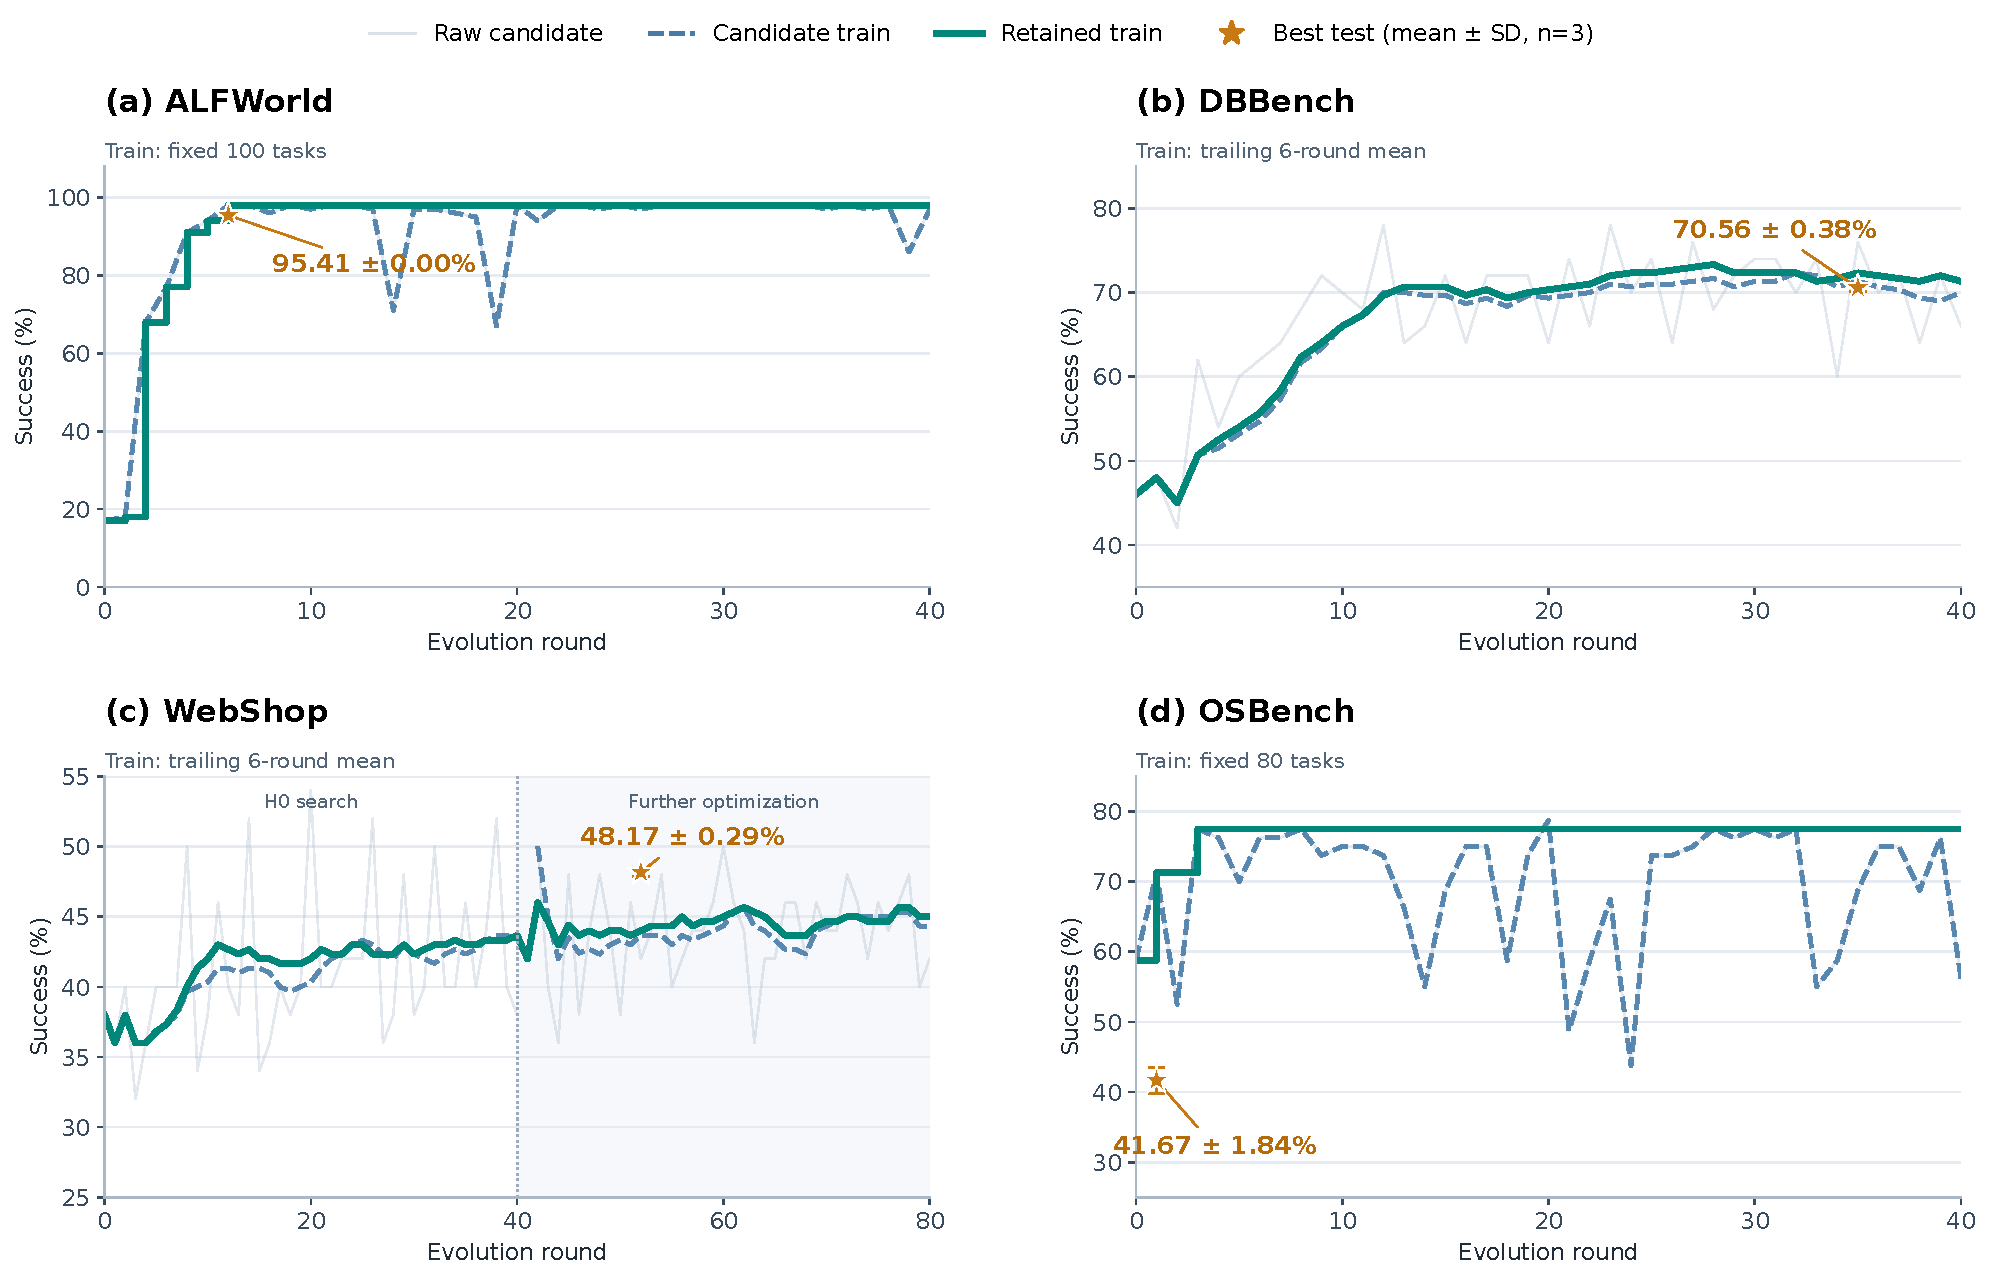
\includegraphics[width=\textwidth]{dsh-draft/figures/appendix-evolution/best-harness-evolution.pdf}
\caption{Evolution of selected high-performing harnesses. All four panels use Sol high with scope C and correspond to the headline checkpoints in Table~\ref{tab:main-results}. Gray lines show raw candidate training scores, blue dashed lines show candidate trends, and green lines show retained training trends. DBBench and WebShop trends use six-round means; ALFWorld and OSBench use fixed-pool scores. Stars show the highest measured test mean with sample SD over three executions. The experimental setup and averaging details are in Appendices~B and D.}
\label{fig:evolution}
\end{figure*}


The evolved harnesses lead the displayed Qwen3-4B comparisons on all four benchmarks (Table~\ref{tab:main-results}). They improve over the local Life-Harness results by 7.64, 6.45, 6.84, and 4.86 percentage points on ALFWorld, DBBench, WebShop, and OSBench, respectively. Relative to the bare Qwen3-4B references, the gains are 78.90, 26.56, 18.67, and 20.17 points. These results establish the quality of the discovered harnesses; the A/B/C comparison below examines how improver capability and editable representation relate to that quality.

Figure~\ref{fig:evolution} complements the endpoint results with candidate and retained training trajectories. The highest measured test checkpoints are marked at their search rounds.



\paragraph{Evolved artifacts.}
Appendix~E presents four artifact architecture figures, each combining a responsibility overview with implementation details. Their structures range from filesystem guidance to receipt-driven action recovery and multi-plugin SQL and shopping mechanisms. Module names, state variables, and intervention points follow the selected checkpoint code.

\subsection*{4.2 Improver by Editable Scope: Nine Configurations}
\begin{figure*}[!t]\centering
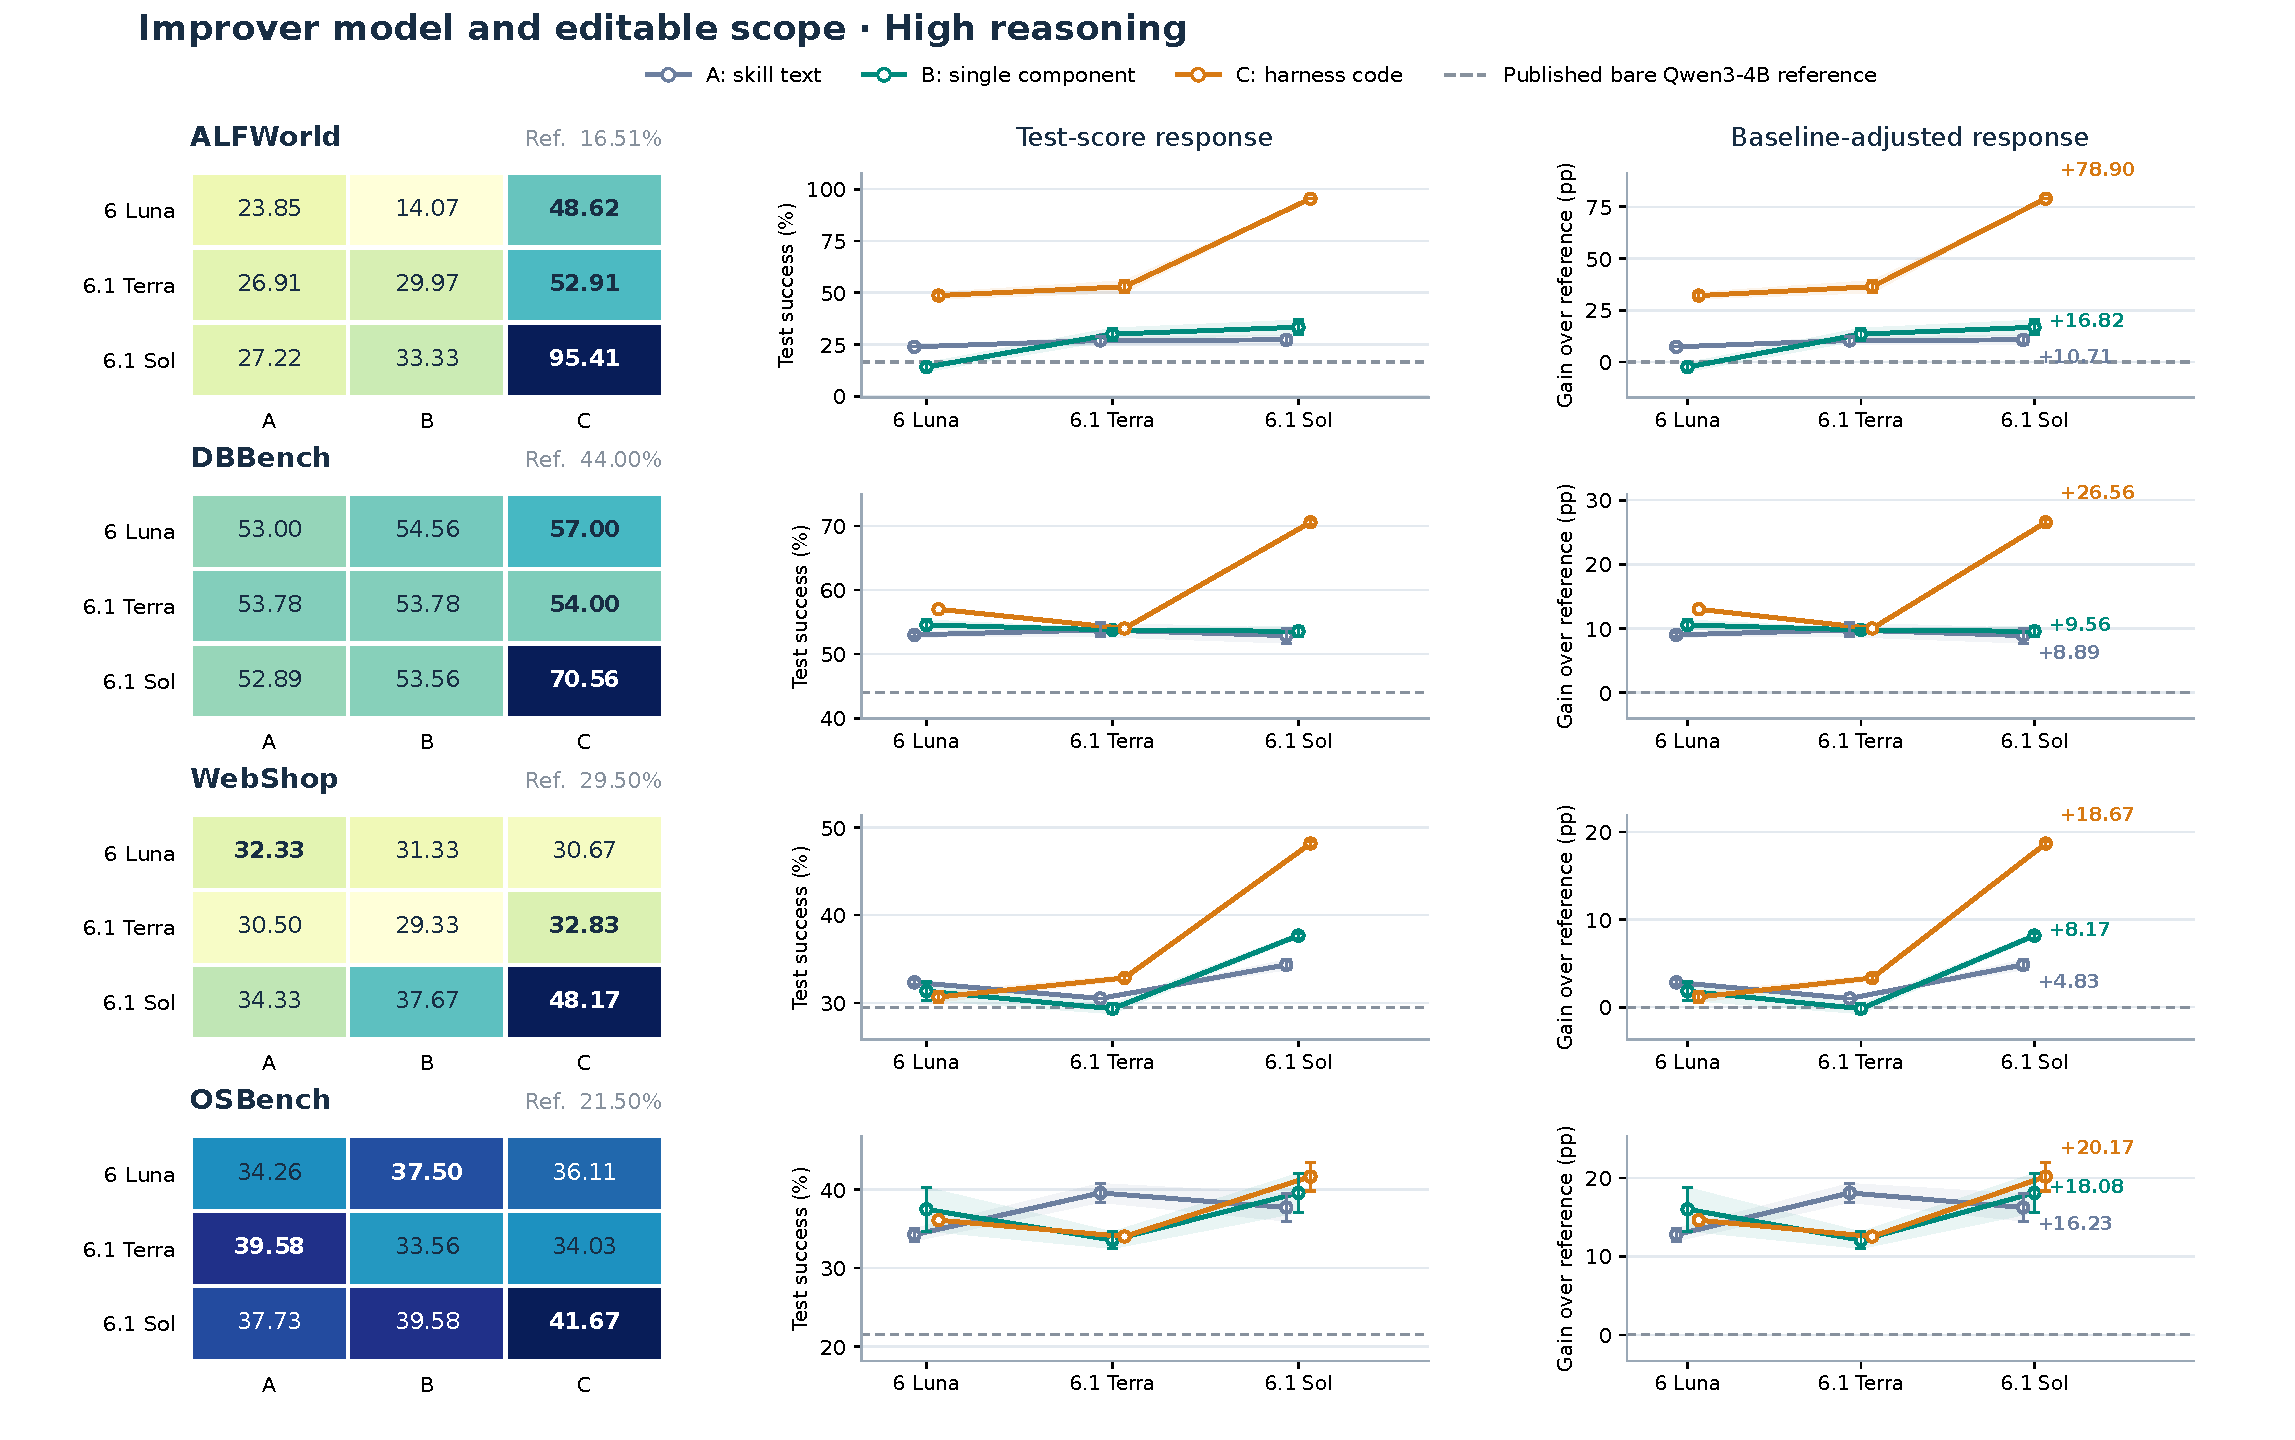
\includegraphics[width=\linewidth]{dsh-draft/figures/combined-comparisons/scope-heatmap-response-gain.pdf}
\caption{Test success across three improvers and edit scopes A/B/C. Heatmaps, score profiles, and gains summarize the same nine model--scope combinations per benchmark. Protocols and metric definitions are in Appendices~B and D.}
\label{fig:scope-overview}\end{figure*}
Figure~\ref{fig:scope-overview} compares three improvers across A, B, and C. We analyze the results along two axes: the benefit of expanding the edit space for a given improver, and the separation between improvers as that space expands.

\paragraph{Expanding the edit space yields the largest gains with Sol.}
Sol's success rates increase from A to B to C on all four benchmarks: 27.22\% $\rightarrow$ 33.33\% $\rightarrow$ 95.41\% on ALFWorld, 52.89\% $\rightarrow$ 53.56\% $\rightarrow$ 70.56\% on DBBench, 34.33\% $\rightarrow$ 37.67\% $\rightarrow$ 48.17\% on WebShop, and 37.73\% $\rightarrow$ 39.58\% $\rightarrow$ 41.67\% on OSBench. Its unweighted mean success across the four benchmarks rises from 38.04\% to 41.03\% to 63.95\%. The largest increment is from B to C, where the improver can construct coordinated mechanisms: the mean increases by 22.92 percentage points. The corresponding A-to-C mean gains are 25.91 points for Sol, 7.24 for Luna, and 5.75 for Terra, calculated from the unrounded scores.

\paragraph{Richer representations amplify the separation between improvers.}
The cross-benchmark means for Luna, Terra, and Sol are 35.86\%, 37.69\%, and 38.04\% in A, compared with 43.10\%, 43.44\%, and 63.95\% in C. Sol's advantage over the better of the other two mean scores expands from 0.35 points in A to 20.51 points in C. The same pattern is visible within benchmarks. On ALFWorld, all three improvers score between 23.85\% and 27.22\% in A; in C, Sol reaches 95.41\%, compared with Luna's 48.62\% and Terra's 52.91\%. On DBBench, Sol moves from 52.89\% in A, slightly below both alternatives, to the leading C score of 70.56\%. Thus, the richer representation exposes a much larger performance difference between improvers.

\paragraph{The joint configuration is the central result.}
Sol with C is the highest-scoring model--scope combination on every benchmark. Luna and Terra obtain smaller and task-dependent gains: for example, Luna moves from 32.33\% to 30.67\% on WebShop, while Terra moves from 39.58\% to 34.03\% on OSBench. This contrast makes the joint design principle concrete. Expanding the editable space creates more candidate directions; a capable improver is needed to turn those directions into effective repairs. The strongest observed configuration combines the broader representation with the improver that uses it most effectively.

\subsection*{4.3 From Search-Space Expansion to Better Harnesses}
\paragraph{Additional dimensions represent additional mechanisms.}
Moving from A to B introduces executable memory, action checks, and receipt processing. Moving to C adds joint choices over their state and dependencies. These degrees of freedom enlarge the space of expressible repairs: a candidate can introduce a fact, the handler that records it, and the later handlers that consume it together. Sol's large B-to-C gains on ALFWorld, DBBench, and WebShop connect the empirical improvement to this expansion of the candidate representation.

\paragraph{Trajectory synthesis supplies a repair direction.}
The algorithm in Section~\ref{sec:method} provides the mechanism for searching this space. The improver receives successful and failed trajectories together with the parent source, runtime interfaces, and the preceding measured decision. It can relate recurring failures to missing state, ineffective guidance, or action-control gaps, while using successful behavior to identify what should be preserved. The resulting attribution specifies a gradient-like direction in discrete program space. Candidate generation turns this direction into an executable update, and paired evaluation determines whether the update improves behavior. Our interpretation of the model--scope results is that stronger trajectory synthesis and candidate design help an improver exploit the additional editable dimensions.

\paragraph{Discovered programs connect evidence to later decisions.}
The artifact structures in Appendix~E show the mechanisms available in this space. ALFWorld's action-hint plugin carries receipt evidence into episode state, subsequent context, and action checks. DBBench combines SQL construction guidance, write tracking, recovery, and result conversion across the execution pipeline. WebShop uses observed page and selection state to guide later search and purchase decisions. These programs illustrate why a repair may require coordinated changes across several stages. OSBench's selected artifact instead uses skill instructions, illustrating that C also retains access to simpler solutions. The expanded space lets the improver choose the form of repair that fits the task. Together, the score profiles and artifact structures support increasing improver capability and edit complexity as complementary directions for harness optimization.
